\section{Stream Processing and its Building blocks}

\subsection{Background}

\begin{itemize}
	\item basic definitions of stream processing. 
	\item what is operator
	\item how do messages flow
	\item how operators are connected
	\item API
\end{itemize}


\subsection{High Level Overview}
\begin{itemize}
	\item describe the main building blocks. These are in Table \ref{table:blocks}
	\item discuss the definition, purpose, importance of each block.	
\end{itemize}


\begin{table}[h]
	%\centering
	\tbl{Essential building blocks in Stream Processing Engines.	\label{table:blocks}}{
		\begin{tabular}{c|l|l}%
			\hline
			\rowcolor[HTML]{E0E0E0} 
			\bfseries Section & \bfseries Building Block & \bfseries Definition  % specify table head
			\csvreader[head to column names]{tables/building-blocks.csv}{}% use head of csv as column names
			{\\\hline\csvcoli&\csvcolii & \csvcoliii}% specify your coloumns here
			\\ \hline
		\end{tabular}
	}
\end{table}

\Fix{Do we want to argue we are covering all essential building blocks??? or just say the most important ones?}




\subsection{Interaction Among Building Blocks}

\begin{itemize}
	\item Draw a figure of the building blocks and their interaction. 
	\item Talk about how the influence each other
	\item Maybe try to break them down into a layers? with some being in a touching-all layer?
\end{itemize}


%

\begin{figure}[h]
	\centering
	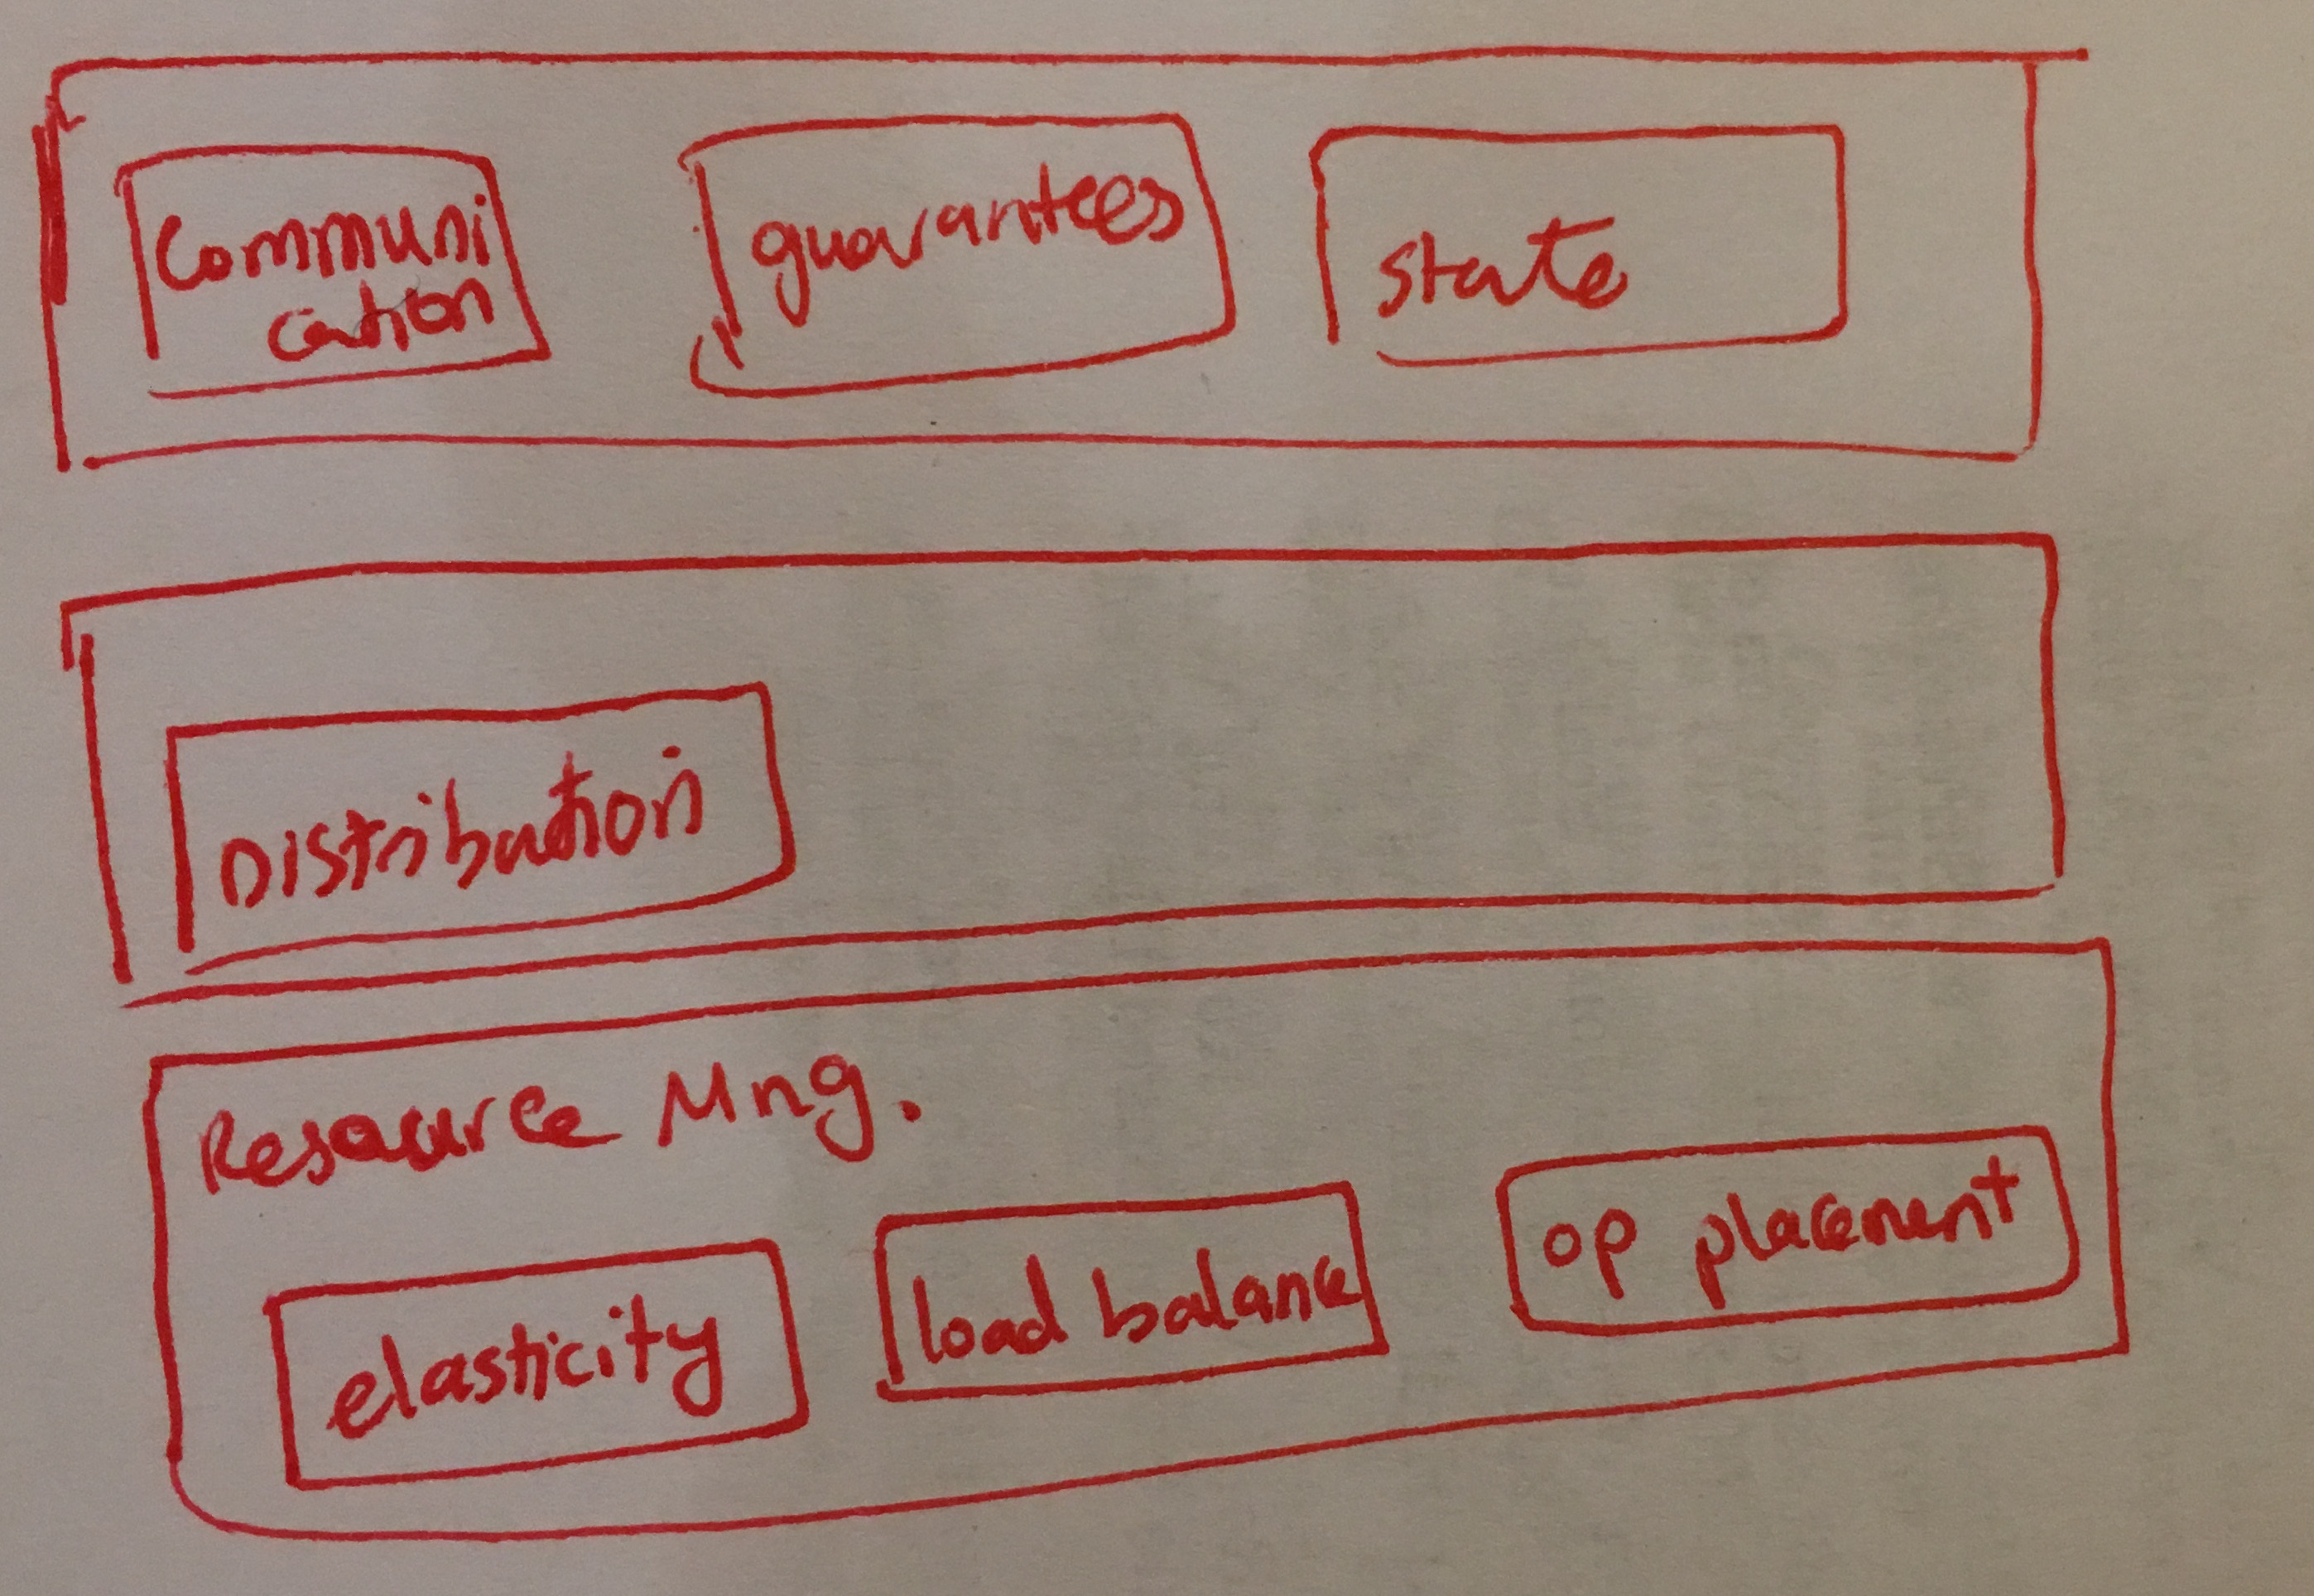
\includegraphics[width=0.45\linewidth]{interaction.jpg}
	\caption{\Fix{Sample figure of how components interact with one another. This is not complete.}}
	\label{fig:tree-cpVScl}
\end{figure}


